\section{Experiments}
\label{sec:experiments}

In the following sections, we present the results of our experiments. We begin by examining the variability and bias in the estimates of the regression coefficients. We then move on to predictive performance and hyperparameter selection. We also consider the effect of class imbalance on the estimates of the regression coefficients. Finally, we look at the effect of interactions between features on the estimates of the regression coefficients.

In all cases where we use simulated data, we generate our response vector according to
\[
  \vec{y} = \mat{X}\vec{\beta}^* + \vec{\varepsilon},
\]
with \(\vec{\varepsilon} \sim \normal(\vec{0}, \sigma_\varepsilon^2 \mat{I})\), where \(\mat{X}\) is the design matrix, \(\vec{\beta}^*\) is the vector of true regression coefficients, and \(\sigma_\varepsilon^2\) is the noise level.

We consider two types of features: binary and quasi-normal features.
To generate binary vectors, sample \(\ceil{qn}\) indexes uniformly at randomly without replacement from \(\{1,2,\dots,n\}\) and set the corresponding elements to one and the remaining ones to zero.
To generate quasi-normal features, we generate a linear sequence \(\vec{w}\) with \(n\) values from  \(10^{-4}\) to \(1 - 10^{-4}\), set
\[
  x_{ij} = \cdf^{-1}(w_i)
\]
and then shuffle the elements of \(\vec{x}_j\) uniformly at random.

In each case, we fit an elastic net model parameterized through \(\lambda_1 = \alpha \lambda\), \(\lambda_2 = (1 - \alpha)\lambda\).

Throughout the experiments, we have used the \pkg{Lasso.jl} package~\citep{kornblith2024} to fit the elastic net, which implements the coordinate descent algorithm~\citep{friedman2010}.
All experiments were coded using the Julia programming language~\citep{bezanson2017} and the code is availabe at \url{XXX}.
% TODO: Add link to reposiory.

\subsection{Variability and Bias in Estimates}

In our first experiment, we consider a simple linear regression model with \(p = 1\,000\) features, out of which the first 20 features correspond to signals, with \(\beta_j^*\) decreasing from 1 to 0.1 linearly.
The class balance of the first 20 features decreases linearly on a log-scale from 0.5 to 0.99.
We estimate the regression coefficients using the lasso and ridge regression and compare the estimates to the true coefficients. The results are shown in~\Cref{fig:binary-decreasing}.

\begin{figure}[htpb]
  \centering
  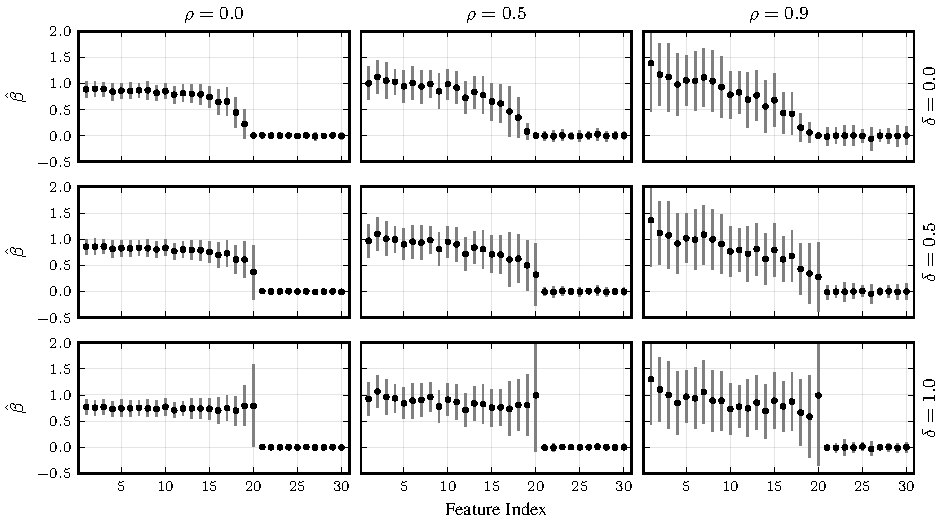
\includegraphics[]{plots/binary_decreasing.pdf}
  \caption{%
    Estimates of the regression coefficients, \(\hat{\vec{\beta}}\), for the first 40 coefficients in the experiment. All of the features are binary and the first 20 features correspond to true signals, with a geometrically decreasing class balance from 0.5 to 0.99. The remaining features have a class balance that's randomly sampled from a uniform distribution with parameters 0.5 and 0.99.}
  \label{fig:binary-decreasing}
\end{figure}






\subsection{Predictive Performance}

\begin{figure}[htpb]
  \centering
  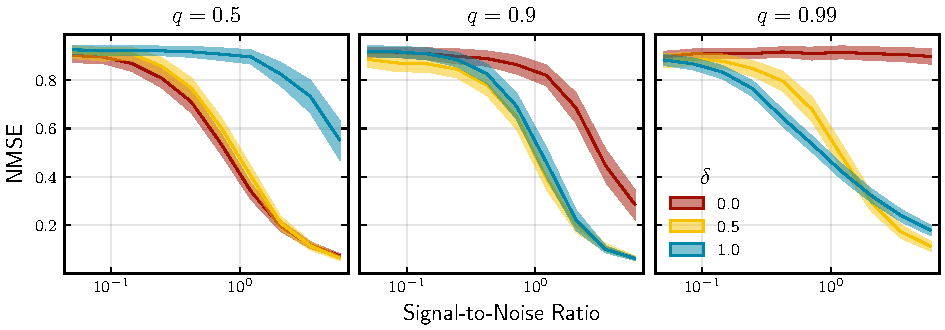
\includegraphics[]{plots/binary_data_sim.pdf}
  \caption{%
    Mean-squared error of \(y - \hat y\) for different types of normalizaion and types of class imbalances in a data set with only binary features.
  }
  \label{fig:binary-sim}
\end{figure}

\subsection{Hyperparameter Selection}

\begin{figure}[htpb]
  \centering
  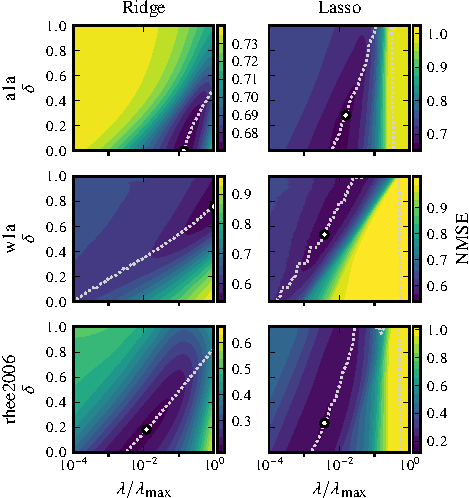
\includegraphics[]{plots/hyperopt_surfaces.pdf}
  \caption{%
    Contour plots of hold-out error across a grid of \(\delta\) and \(\lambda\) values for the
    lasso.
  }
  \label{fig:hyperopt-contours}
\end{figure}

\begin{figure}[htpb]
  \centering
  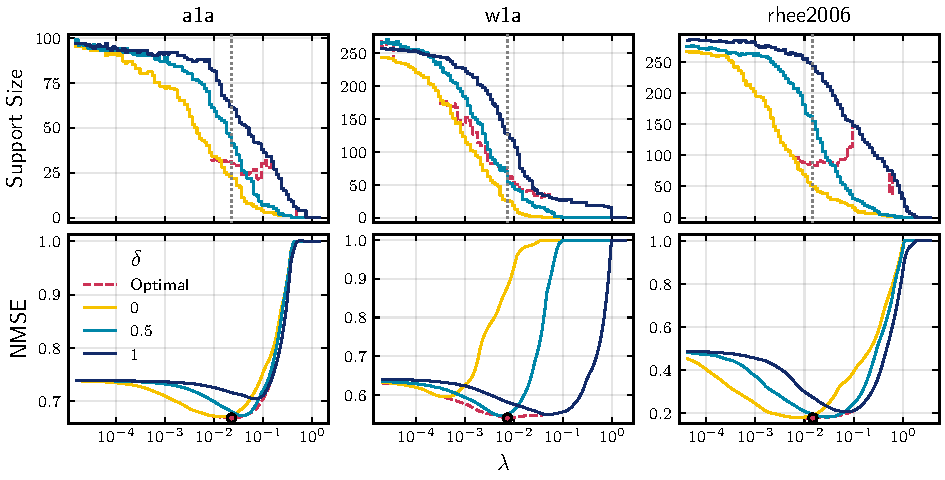
\includegraphics[]{plots/hyperopt_paths.pdf}
  \caption{%
    Support and NMSE of the lasso for different values of \(\delta\) and \(\lambda\).
  }
  \label{fig:hyperopt-support}
\end{figure}

\subsection{Mixed Data}

The next question we now ask ourselves is: given that both features are in the model, what are their respective sizes given differences in class balance (\(q\))?

To begin to answer this question, we conduct simulations on a two-dimensional problem. Along with our previous reasoning, we sample one feature from \(\normal(0, 0.5)\) and the other from \(\bernoulli(q)\), varying \(q\) in \([0.5, 0.99]\) to simulate the effect of class imbalance on the estimates from the model.

The results~(\Cref{fig:lasso-ridge-comparison}) show that when it comes to ridge, standardization creates class balance-insensitive estimates, whereas for the lasso, this is not the case. For the lasso, it is instead the Mean-StdVar and Mean-Var normalization methods that generate estimates that are insensitive to class imbalances.

\begin{figure}[htpb]
  \centering
  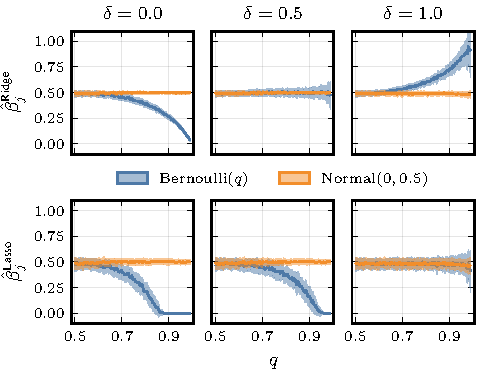
\includegraphics{plots/mixed_data.pdf}
  \caption{%
    Comparison between lasso and ridge estimators for a two-dimensional problem where one feature is generated from \(\bernoulli(q)\) and the other from \(\normal(0, 0.5)\) and the features are normalized in various ways.}
  \label{fig:lasso-ridge-comparison}
\end{figure}

\subsection{Interactions}

\begin{figure}[htpb]
  \centering
  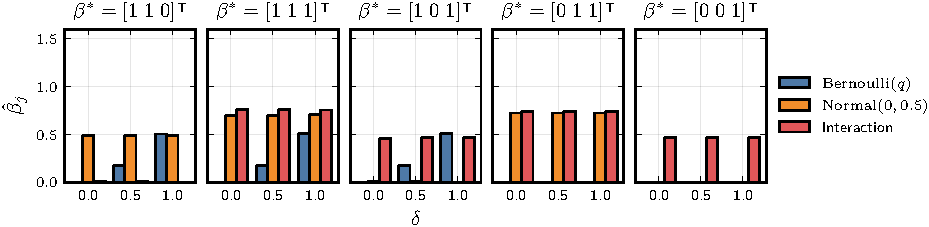
\includegraphics[]{plots/interactions.pdf}
  \caption{%
    The effect of different normalization strategies for mixed data with interactions.
  }
\end{figure}
